
\item {\bf Reinforcement Learning: Policy Gradient}

In this problem, you will implement the REINFORCE policy gradient algorithm to optimize on a stochastic policy that solves a simple gridded environment.\\

\textbf{The Environment}

In this problem, we will explore the Grid World environment, implemented in {\tt Grid\_World.py}.  This provides a gridded rectangular world of cells, each of which has an associated reward.  In each cell, the agent can perform one of four actions: [RIGHT, UP, LEFT, DOWN].  The episode is terminated when the agent enters one of the termination cells.  You should feel free to experiment with different Grid World setups, but you will be graded on the one shown below.  In this 5x5 environment, the agent always starts at the top left corner (0,0).  There is a -1 reward at the bottom left corner (4,0) and a +1 reward at the top right corner (0,4).  All other cells have a reward of zero.  The non-zero reward cells ((0,4) and (4,0)) are also termination cells- the episode ends when the agent lands in one of these cells.

\begin{center}
  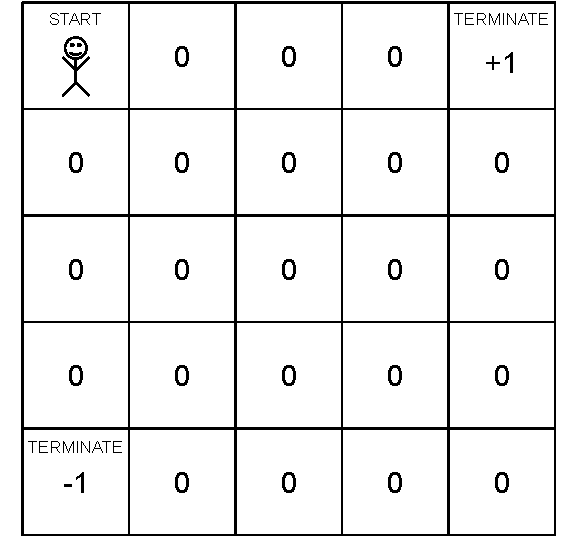
\includegraphics[width=8cm]{policy-gradient/Grid_World.pdf}
\end{center}

Your policy must learn to maximize reward in the Grid World, which for the above environment means to travel to the top right cell as quickly as possible.\\

\textbf{Policy Gradient}

Below is the REINFORCE algorithm derived in lecture.  Note that any policy will work with this algorithm, as long as it is differentiable and results in a probability distribution over all possible actions.  For simplicity, we will grade you on your implementation of the softmax policy.  The steps below will guide you through deriving the update step for a softmax policy.

{\tt
Loop:\\
\-\ Sample: $(s_0, a_0), (s_1, a_1),...$\\
\-\ Compute Payoff: payoff $=R(s_0)+R(s_1)+...$\\
\-\ Update Weights: $\theta\coloneqq\theta+\alpha\left[\frac{\nabla_\theta\pi_\theta(s_0,a_0)}{\pi_\theta(s_0,a_0)}+\frac{\nabla_\theta\pi_\theta(s_1,a_1)}{\pi_\theta(s_1,a_1)}+...\right]$(payoff)}\\

Let's take a look at the payoff term.  In lecture, we presented the case of a non-discounted MDP payof.  However, REINFORCE tends to converge better in the discounted case.  This is because transitions closer to a reward have a higher impact on the weight update.  To calculate the discounted payoff, notice that each step must now have a different payoff, which we will call $G_t$:

$$\theta\coloneqq\theta+\alpha\left[G_0\frac{\nabla_\theta\pi_\theta(s_0,a_0)}{\pi_\theta(s_0,a_0)}+G_1\frac{\nabla_\theta\pi_\theta(s_1,a_1)}{\pi_\theta(s_1,a_1)}+...\right]$$

To calculate $G_t$, consider a simple episode with five steps, each earning a reward of zero except the final step, which earns a reward of one:

$$R=\left[0,0,0,0,1\right]$$

Applying a discount factor $\gamma=0.9$, we can calculate the following discounted sum of future rewards:
\begin{align*}
G&=\left[\gamma^4, \gamma^3, \gamma^2, \gamma^1, 1\right]\\
 &=\left[0.66, 0.73, 0.81, 0.9, 1\right]
\end{align*}

Here you can see that early transitions are given less payoff, which is intuitive since they likely had less impact on achieving the later reward.  To calculate $G_t$ in any series of rewards, use the formal definition below (using initial timestep $t$ and reference future timestep $k$).  This is known as the {\bf discounted sum of future rewards} or the {\bf discounted return}.

\begin{align*}
    G_t &= R_t + \gamma R_{t+1} + \gamma^2 R_{t+2} + \gamma^3 R_{t+3} + ...\\
    &=\sum^{T-1}_{k=t}\gamma^{k-t}R_k
\end{align*}

We will now walk through deriving the policy gradient for a softmax policy (part (a)), then implement the REINFORCE algorithm in practice to solve Grid World (part (b)).

\begin{enumerate}
  \input{policy-gradient/01-softmax_gradient}

  \item \points{1b}

Now, implement the REINFORCE algorithm by completing the missing code within {\tt REINFORCE.py}.  The partially completed functions contain additional help and instructions.  When you have correctly implemented the required code, run the REINFORCE algorithm with the following command {\tt python train.py}.  This will train many agents (default is 20) using REINFORCE on the Grid World, then save the visualized results, averaged over all the trained agents, to {\tt policy\_gradient\_results.pdf}.  A correct implementation will look similar to the image below.

\begin{center}
  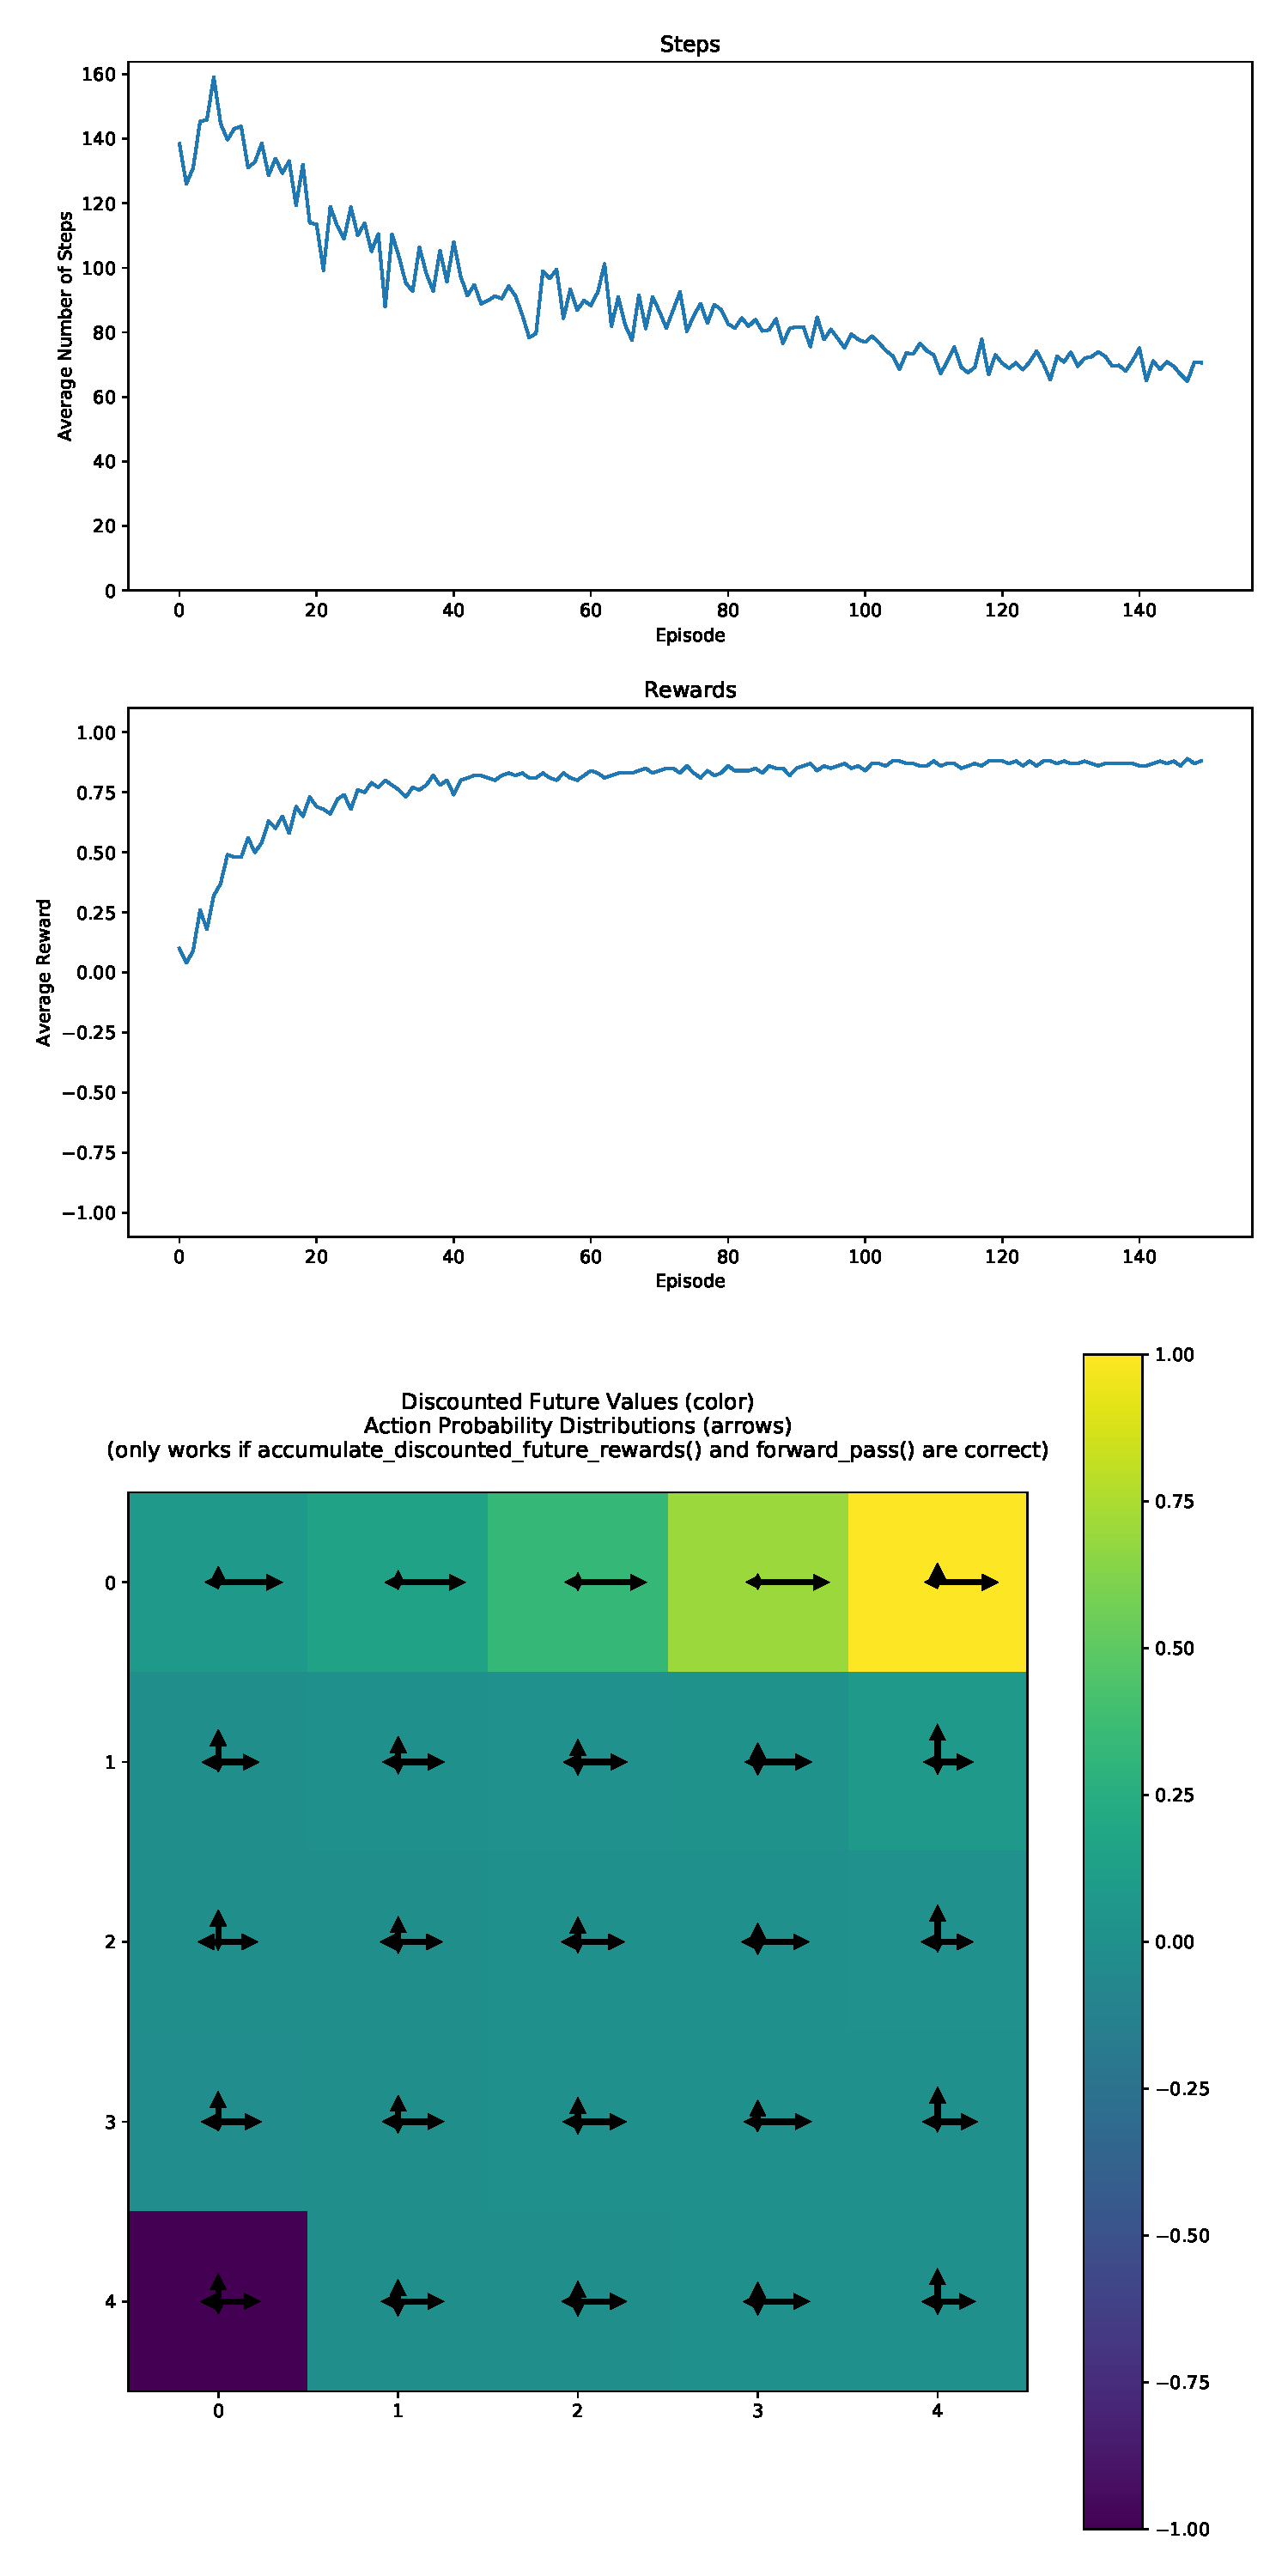
\includegraphics[width=12cm]{policy-gradient/policy_gradient_results.pdf}
\end{center}


\end{enumerate}
